%!TEX root = ../nyu021114.tex

% background on genotype-phenotype maps
% folder name: GPmaps

\begin{frame}
\vspace{1em}
\frametitle{Coarse-graining of gene expression data}
\begin{center}
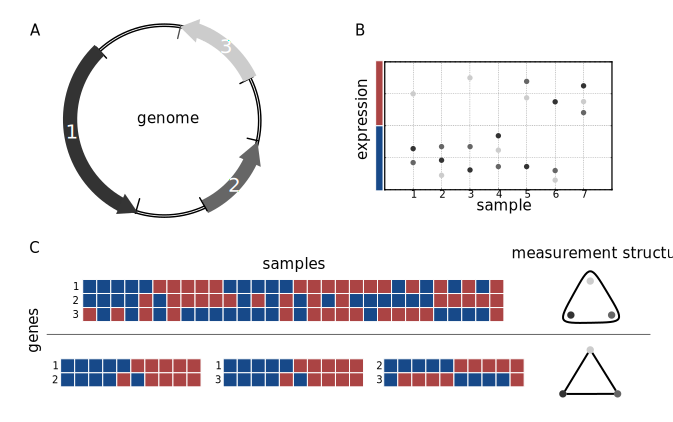
\includegraphics[width=0.8\textwidth]{fig/figure_expression_concept.pdf}\\
%\hfill \cite{Elowitz2000b}
\end{center}
\end{frame}

\begin{frame}
\vspace{1em}
\frametitle{Probabilistic graphical model of inconsistent gene expression data}
\begin{center}
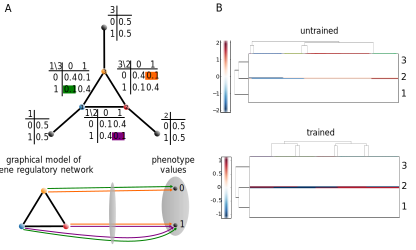
\includegraphics[width=0.8\textwidth]{fig/inconsistentthreecycle.pdf}\\
%\hfill \cite{Elowitz2000b}
\end{center}
\end{frame}

\begin{frame}
\vspace{1em}
\frametitle{Relationship between gene regulatory network models and spaces of probability distributions}
\begin{center}
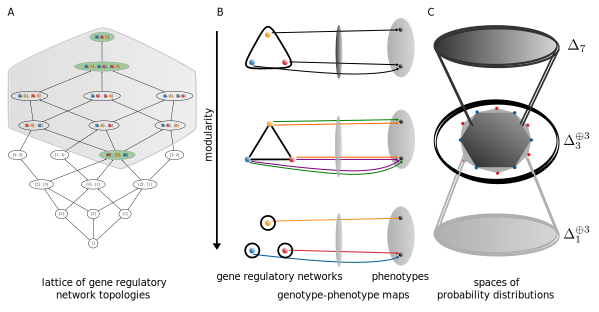
\includegraphics[width=0.9\textwidth]{fig/conediagram.pdf}\\
%\hfill \cite{Elowitz2000b}
\end{center}
\end{frame}

\begin{frame}
\vspace{1em}
\frametitle{Hierarchical relationships among all possible classes of hypergraphs that are not graphs (i.e. not 2-uniform) but have cycles}
\begin{center}
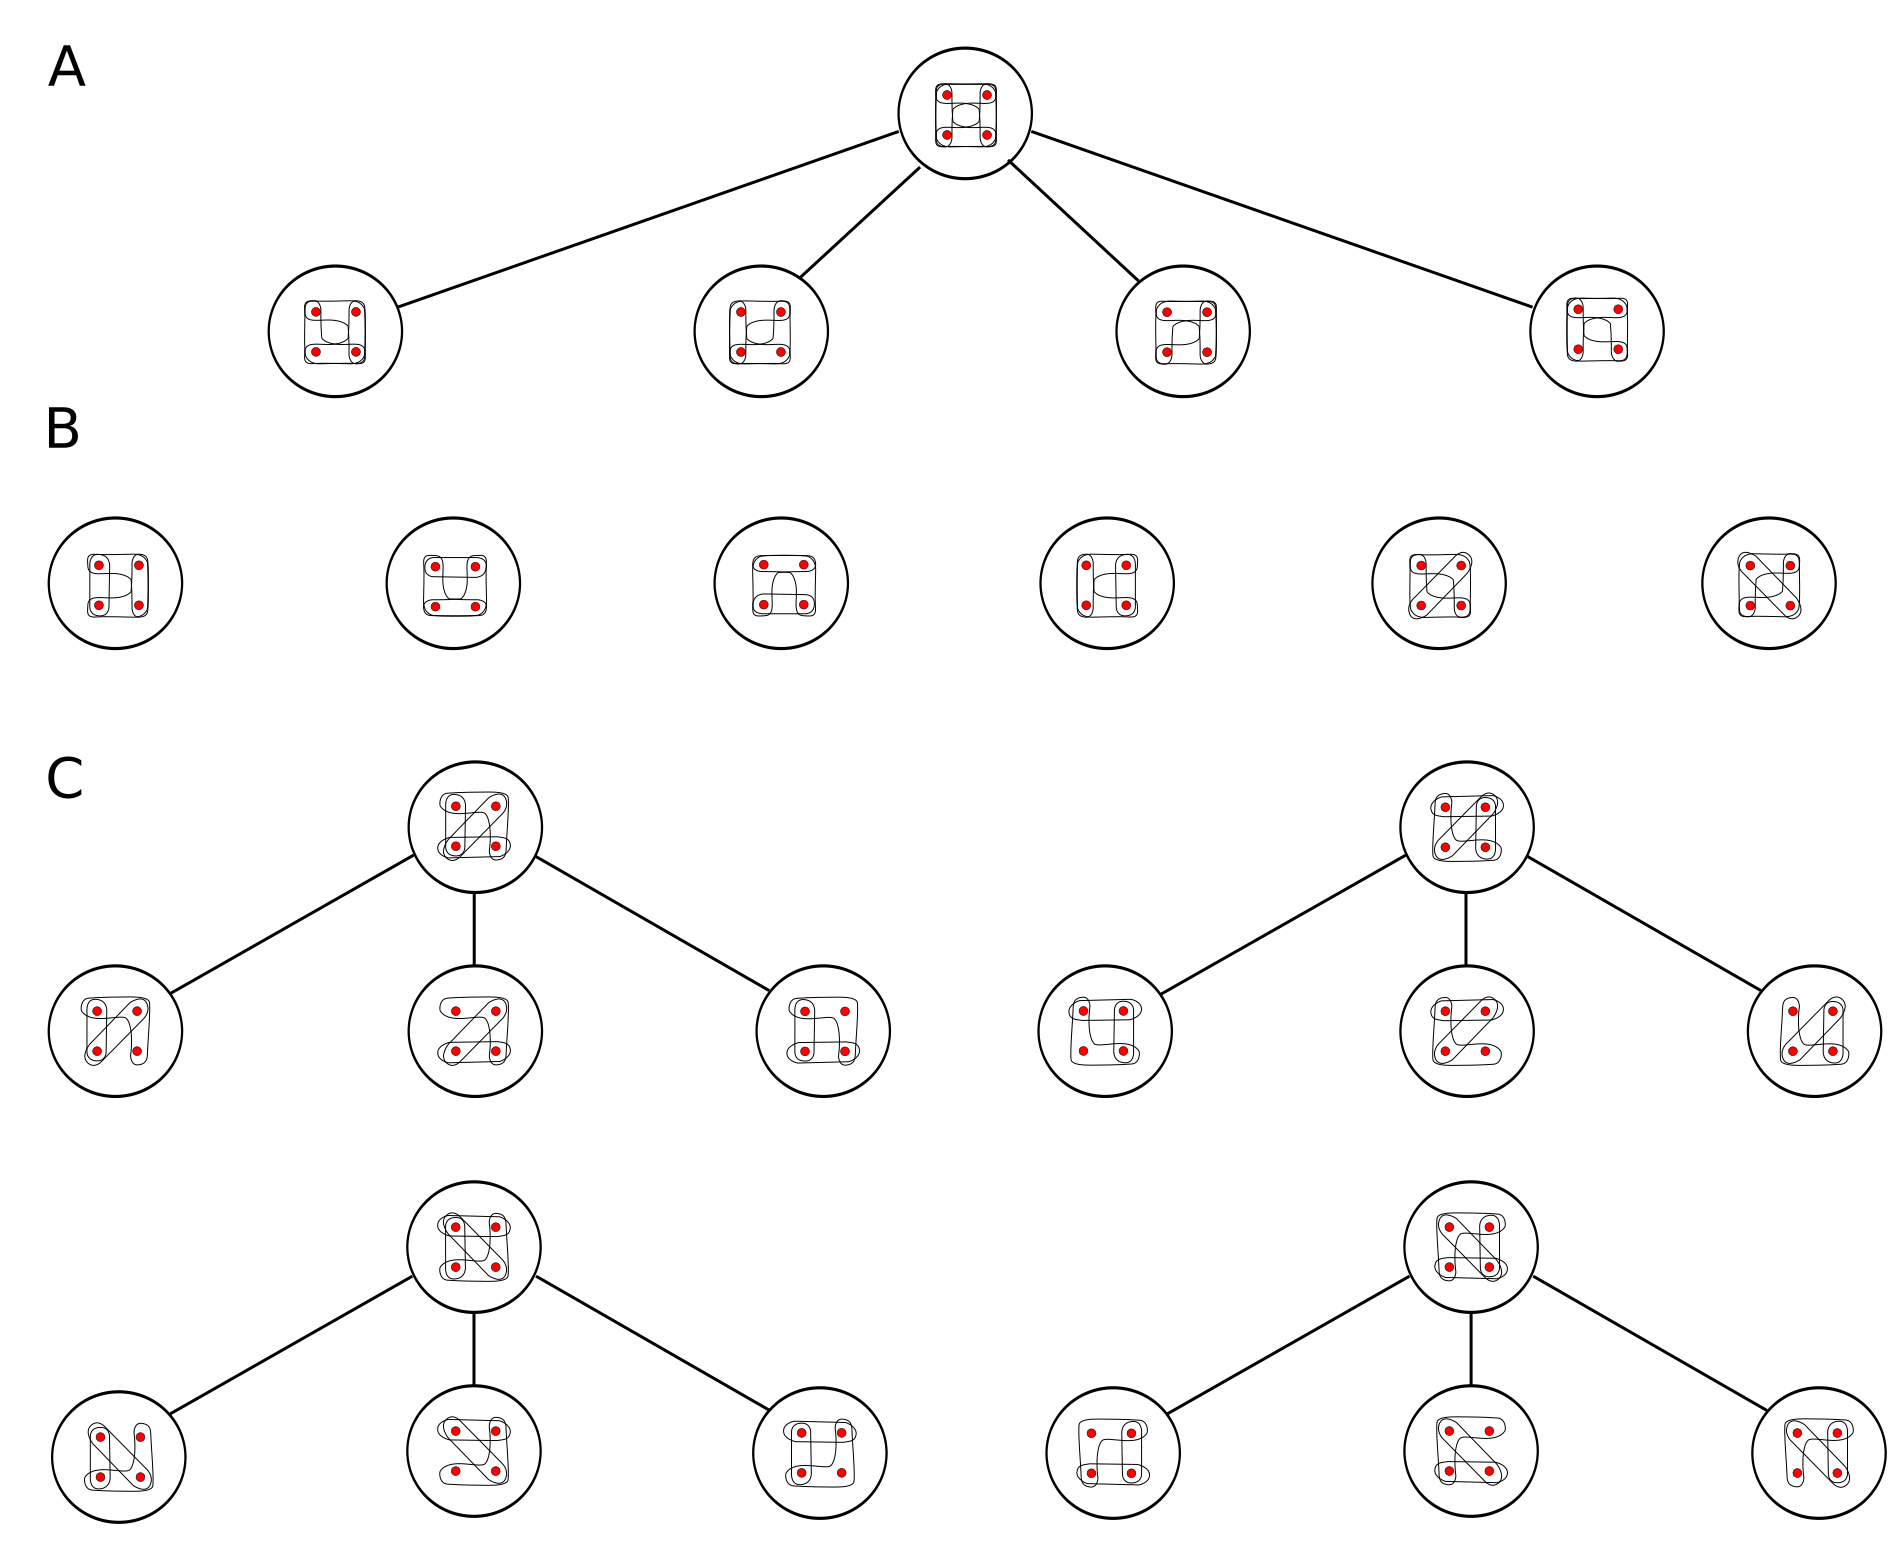
\includegraphics[width=0.7\textwidth]{fig/non2uniformcyclichypergraphhasse.pdf}\\
%\hfill \cite{Elowitz2000b}
\end{center}
\end{frame}

\begin{frame}
\vspace{1em}
\frametitle{Non-modular to modular probability space volume ratio}
\begin{center}
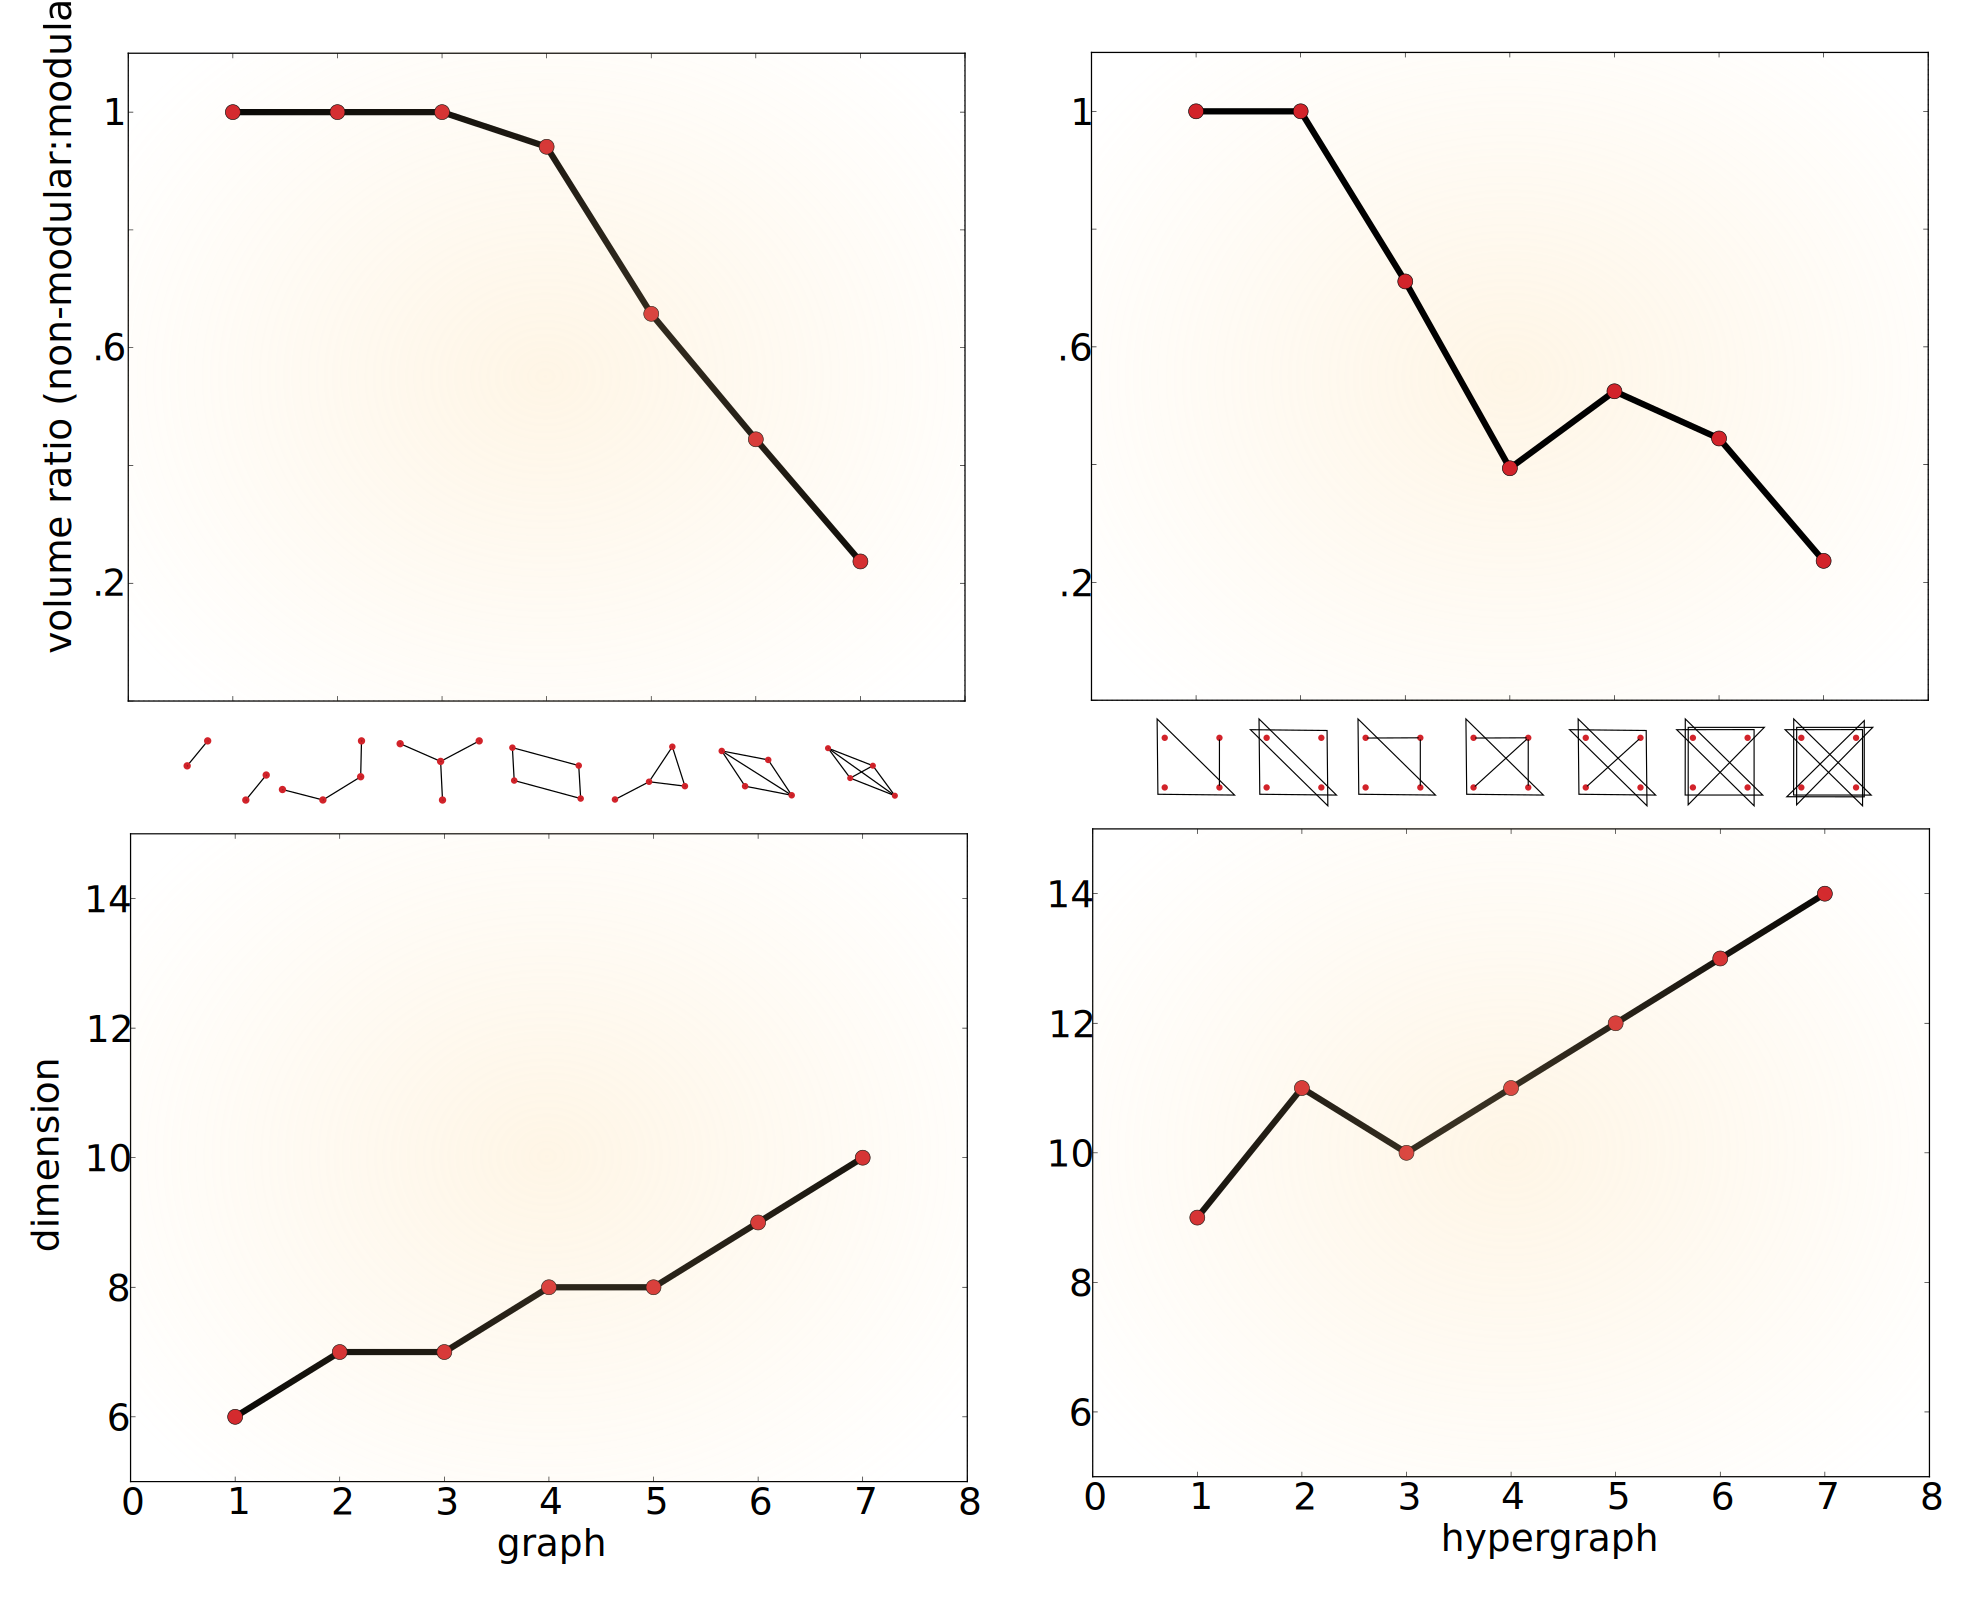
\includegraphics[width=0.8\textwidth]{fig/figure_graphs_dims_nolines.pdf}\\
%\hfill \cite{Elowitz2000b}
\end{center}
\end{frame}

\begin{frame}
\vspace{1em}
\frametitle{Schematic representation of the constraints imposed on stochastic gene expression and evolutionary dynamics by network architecture}
\begin{center}
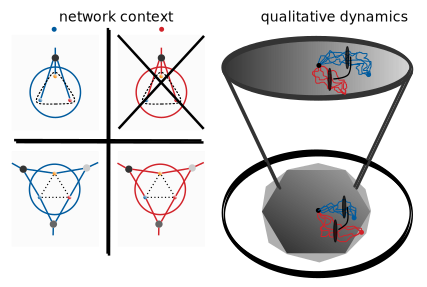
\includegraphics[width=0.6\textwidth]{fig/stochdynscheme.pdf}\\
%\hfill \cite{Elowitz2000b}
\end{center}
\end{frame}
